\graphicspath{{./img/}}
\onehalfspacing
\section{Đề số 4}

\begin{bt} 
   \hfill
   \begin{enumerate}[a.]
    \item Thực hiện phép tính: $\mathrm{A}=\left[\left(\frac{2}{193}-\frac{3}{386}\right) \cdot \frac{193}{17}+\frac{33}{34}\right]:\left[\left(\frac{7}{1931}+\frac{11}{3862}\right) \cdot \frac{1931}{25}+\frac{9}{2}\right]$.
    \item Rút gọn :    
    $$
    \mathrm{B}=(-5)^0+(-5)^1+(-5)^2+(-5)^3+\ldots+(-5)^{2016}+(-5)^{2017}
    $$
   \end{enumerate}
\loigiai{
    \begin{enumerate}
        \item
        $$
        \begin{aligned}
        & \bullet\left[\left(\frac{2}{193}-\frac{3}{386}\right) \cdot \frac{193}{17}+\frac{33}{34}\right]=\frac{2}{193} \cdot \frac{193}{17}-\frac{3}{386} \cdot \frac{193}{17}+\frac{33}{34}=\frac{2}{17}-\frac{3}{34}+\frac{33}{34}=1 \\
        & \bullet\left[\left(\frac{7}{1931}+\frac{11}{3862}\right) \cdot \frac{1931}{25}+\frac{9}{2}\right]=\frac{7}{1931} \cdot \frac{1931}{25}+\frac{11}{3862} \cdot \frac{1931}{25}+\frac{9}{2}=\frac{7}{25}+\frac{11}{50}+\frac{9}{2}=5 \\
        & \mathrm{~A}=1: 5=\frac{1}{5}
        \end{aligned}
        $$
        \item
        $$
        \begin{aligned}
        (-5) \mathrm{B} & =(-5)^1+(-5)^2+(-5)^3+\ldots+(-5)^{2016}+(-5)^{2017}+(-5)^{2018} . \\
        \mathrm{B} & =(-5)^0+(-5)^1+(-5)^2+(-5)^3+\ldots+(-5)^{2016}+(-5)^{2017} .
        \end{aligned}
        $$
        Do đó: $(-5) \mathrm{B}-\mathrm{B}=(-6) \mathrm{B}=(-5)^{2018}-1$
        $$
        \text { Vậy } B=\frac{(-5)^{2018}-1}{-4}=\frac{1-5^{2018}}{4}
        $$
    \end{enumerate}
} 
\end{bt}

\begin{bt}
    \hfill
    \begin{enumerate}[a.]
        \item Tìm a, b, c biết $\quad \frac{12 a-15 b}{7}=\frac{20 c-12 a}{9}=\frac{15 b-20 c}{11}$ và $a+b+c=48$.
        \item Một công trường dự định phân chia số đất cho ba đội I, II, III tỉ lệ với 7; 6; 5 . Nhưng sau đó vì số người của các đội thay đổi nên đã chia lại tỉ lệ với $6 ; 5 ; 4$. Như vậy có một đội làm nhiều hơn so với dự định là $6 \mathrm{m}^3$ đất. Tính tổng số đất đã phân chia cho các đội.
    \end{enumerate}
\loigiai{
    \begin{enumerate}
        \item Áp dụng tính chất của dãy tỉ số bằng nhau, ta có:\\
        $$
\begin{aligned}
& \frac{12 a-15 b}{7}=\frac{20 c-12 a}{9}=\frac{15 b-20 c}{11}=\frac{12 a-15 b+20 c-12 a+15 b-20 c}{27}=0 \\
& \left.\begin{array}{l}
\frac{12 \mathrm{a}-15 \mathrm{~b}}{7}=0 \Rightarrow 12 \mathrm{a}=15 \mathrm{~b} \\
\frac{20 \mathrm{c}-12 \mathrm{a}}{9}=0 \Rightarrow 20 \mathrm{c}=12 \mathrm{a}
\end{array}\right\} \Rightarrow 12 \mathrm{a}=15 \mathrm{~b}=20 \mathrm{c} \Rightarrow \frac{\mathrm{a}}{\frac{1}{12}}=\frac{\mathrm{b}}{\frac{1}{15}}=\frac{\mathrm{c}}{\frac{1}{20}} \\
&
\end{aligned}
$$
Áp dụng tính chất của dãy tỉ số bằng nhau và $\mathrm{a}+\mathrm{b}+\mathrm{c}=48$, ta có:
$$
\begin{aligned}
& \frac{\mathrm{a}}{\frac{1}{12}}=\frac{\mathrm{b}}{\frac{1}{15}}=\frac{\mathrm{c}}{\frac{1}{20}}=\frac{\mathrm{a}+\mathrm{b}+\mathrm{c}}{\frac{1}{12}+\frac{1}{15}+\frac{1}{20}}=\frac{48}{\frac{1}{5}}=24 \\
& \frac{\mathrm{a}}{\frac{1}{12}}=240 \Rightarrow \mathrm{a}=20 \frac{\mathrm{b}}{\frac{1}{15}}=240 \Rightarrow \mathrm{b}=16 \frac{\mathrm{c}}{\frac{1}{20}}=240 \Rightarrow \mathrm{c}=12
\end{aligned}
$$
Vậy $a=20 ; b=16 ; c=12$.
\item Gọi tổng số đất đã phân chia cho các đội là $x\left(\mathrm{~m}^3\right)$ ĐK: $x>0$.\\
Số đất dự định chia cho ba đội I, II, III lần lượt là a, b, c $\left(\mathrm{m}^3\right)$ ĐK: $a, b, c>0$.\\
Ta có: $\frac{a}{7}=\frac{b}{6}=\frac{c}{5}=\frac{a+b+c}{18}=\frac{x}{18} \Rightarrow a=\frac{7 x}{18} ; b=\frac{6 x}{18} ; c=\frac{5 x}{18}$\\
Số đất sau đó chia cho ba đội I, II, III lần lượt là $a^{\prime}, b^{\prime}, c^{\prime}\left(m^3\right)$ ĐK: $a^{\prime}, b^{\prime}, c^{\prime}>0$.\\
Ta có: $\frac{a^{\prime}}{6}=\frac{b^{\prime}}{5}=\frac{c^{\prime}}{4}=\frac{a^{\prime}+b^{\prime}+c^{\prime}}{15}=\frac{x}{15} \Rightarrow a^{\prime}=\frac{6 x}{15} ; b^{\prime}=\frac{5 x}{15} ; c^{\prime}=\frac{4 x}{15}$\\
So sánh (1) và (2) ta có: $a<a^{\prime} ; b=b^{\prime} ; c>c^{\prime}$ nên đội I nhận nhiều hơn lúc đầu.\\
Vi a $-\mathrm{a}^{\prime}=6$ hay $\frac{7 x}{18}-\frac{6 x}{15}=6 \Rightarrow \frac{x}{90}=4 \Rightarrow x=360$\\
Vậy tổng số đất đã phân chia cho các đội là $360 \mathrm{~m}^3$ đất.
    \end{enumerate}
} 
\end{bt}

\begin{bt}
   \hfill
   \begin{enumerate}[a.]
    \item Tìm giá trị nhỏ nhất của biểu thức: $C=\frac{|x-2017|+2018}{|x-2017|+2019}$.
    \item Chứng tỏ rằng $\mathrm{S}=\frac{3}{4}+\frac{8}{9}+\frac{15}{16}+\ldots+\frac{\mathrm{n}^2-1}{\mathrm{n}^2}$ không là số tự nhiên với mọi $\mathrm{n} \in \mathrm{N}, \mathrm{n}>$2.
    \item Tìm tất cả các cặp số nguyên $x$, $y$ sao cho: $x-2 x y+y=0$.
   \end{enumerate}
\loigiai{
    \begin{enumerate}
        \item $C=\frac{|x-2017|+2018}{|x-2017|+2019}=\frac{(|x-2017|+2019)-1}{|x-2017|+2019}=1-\frac{1}{|x-2017|+2019}$\\
        Biểu thức $\mathrm{C}$ đạt giá trị nhỏ nhất khi $|x-2017|+2019$ có giá trị nhỏ nhất\\
        Mà $|x-2017| \geq 0$ nên $|x-2017|+2019 \geq 2019$.
        Dấu "=" xảy ra khi $x=2017 \Rightarrow C=\frac{2018}{2019}$.\\
        Vậy giá trị nhỏ nhất của C là $\frac{2018}{2019}$ khi $x=2017$.
        \item Ta có: \\ 
        $$
\begin{aligned}
& \mathrm{S}=\frac{3}{4}+\frac{8}{9}+\frac{15}{16}+\ldots+\frac{n^2-1}{n^2}=\frac{2^2-1}{2^2}+\frac{3^2-1}{3^2}+\frac{4^2-1}{4^2}+\ldots+\frac{n^2-1}{n^2} \\
& =1-\frac{1}{2^2}+1-\frac{1}{3^2}+1-\frac{1}{4^2}+\ldots+1-\frac{1}{n^2} \\
& =(1+1+1+\ldots+1)-\left(\frac{1}{2^2}+\frac{1}{3^2}+\frac{1}{4^2}+\ldots+\frac{1}{n^2}\right) \\
& =(n-1)-\left(\frac{1}{2^2}+\frac{1}{3^2}+\frac{1}{4^2}+\ldots+\frac{1}{n^2}\right) \\
& \Rightarrow \mathrm{S}<\mathrm{n}-1(1)
\end{aligned}
$$
Nhận xét: $\frac{1}{2^2}<\frac{1}{1.2} ; \frac{1}{3^2}<\frac{1}{2.3} ; \frac{1}{4^2}<\frac{1}{3.4} ; \ldots ; \frac{1}{n^2}<\frac{1}{(n-1) \cdot n}$
$$
\begin{aligned}
& \Rightarrow \frac{1}{2^2}+\frac{1}{3^2}+\frac{1}{4^2}+\ldots+\frac{1}{n^2}<\frac{1}{1.2}+\frac{1}{2 \cdot 3}+\frac{1}{3 \cdot 4}+\ldots+\frac{1}{(n-1) \cdot n}=1-\frac{1}{n}<1 . \\
& \Rightarrow-\left(\frac{1}{2^2}+\frac{1}{3^2}+\frac{1}{4^2}+\ldots+\frac{1}{n^2}\right)>-1 \Rightarrow(n-1)-\left(\frac{1}{2^2}+\frac{1}{3^2}+\frac{1}{4^2}+\ldots+\frac{1}{n^2}\right)>(\mathrm{n}-1)-1 \\
&=\mathrm{n}-2 . \\
& \Rightarrow \mathrm{S}>\mathrm{n}-2(2)
\end{aligned}
$$
Từ (1) và (2) suy ra $\mathrm{n}-2<\mathrm{S}<\mathrm{n}-1$ hay $\mathrm{S}$ không là số nguyên.
\item Ta có:
$x-2 x y+y=0$ \\
$\Rightarrow x(1-y)+y=0$ \\
$\Rightarrow(1-y)+x(1-y)=1$ \\
$\Rightarrow(1+x)(1-y)=1$\\
Ta có $: 1=1 \cdot 1=(-1) \cdot(-1)$\\
Ta có bảng:\\
\begin{tabular}{|c|c|c|}
\hline $1+x$ & 1 & -1 \\
\hline $1-y$ & 1 & -1 \\
\hline $x$ & 0 & -2 \\
\hline $y$ & 0 & 2 \\
\hline
\end{tabular}\\
Vậy $(x ; y) \in\{(0 ; 0) ;(-2 ; 2)\}$
    \end{enumerate}
} 
\end{bt}

\begin{bt}
    Cho tam giác cân $A B C, A B=A C$. Trên cạnh $B C$ lấy điểm $D$, trên tia đối của $C B$ lấy điểm $\mathrm{E}$ sao cho $\mathrm{BD}=\mathrm{CE}$. Các đường thẳng vuông góc với $\mathrm{BC}$ kẻ từ $\mathrm{D}$ và $\mathrm{E}$ cắt $\mathrm{AB}$ và $A C$ lân lượt ở $M$ và $N$. Chứng minh rằng: 
    \begin{enumerate}[a.]
    \item $\mathrm{DM}=\mathrm{EN}$.
    \item Đường thẳng $\mathrm{BC}$ cắt $\mathrm{MN}$ tại điểm $\mathrm{I}$ là trung điểm của $\mathrm{MN}$.
    \item Đường thẳng vuông góc với $\mathrm{MN}$ tại I luôn luôn đi qua một điểm cố định khi $\mathrm{D}$ thay đổi trên cạnh BC.
    \end{enumerate}
\loigiai{
    GT:
    \begin{enumerate}[1.]
        \item $\triangle \mathrm{ABC}$
        \item $\mathrm{AB}=\mathrm{AC}$
        \item $\mathrm{BD}=\mathrm{CE}$
        \item $\mathrm{MD} \perp \mathrm{BC} ; \mathrm{NE} \perp \mathrm{BC} $
        \item $\mathrm{BC} \cap \mathrm{MN}=\{\mathrm{I}\}$
    \end{enumerate}
       
    KL:
    \begin{enumerate}
        \item $\mathrm{DM}=\mathrm{EN}$
        \item Đường thẳng $\mathrm{BC}$ cắt $\mathrm{MN}$ tại điểm I là trung điểm của $\mathrm{MN}$
        \item Đường thẳng vuông góc với $\mathrm{MN}$ tại I luôn luôn đi qua một điểm cố định khi D thay đối trên cạnh BC
    \end{enumerate}
    $$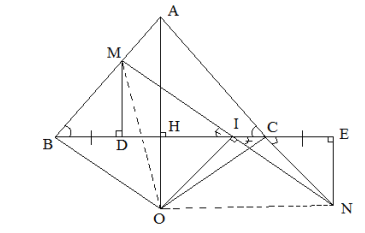
\includegraphics[width=0.55\textwidth]{4-4-lg.png}$$
    \begin{enumerate}
        \item $\triangle \mathrm{MDB}=\triangle \mathrm{NEC}$ (g.c.g)\\
        $\Rightarrow \mathrm{DM}=\mathrm{EN}$ (cặp cạnh tương ứng)\\
        $\Rightarrow \mathrm{MB}=\mathrm{NC}$ (cặp cạnh tương ứng)\\
        \item Ta có:\\
        $\triangle \mathrm{MDI}$ vuông tại $\mathrm{D}: \mathrm{DMI}+\mathrm{MID}=90^{\circ}$ (tổng hai góc nhọn trong tam giác vuông)\\
        $\triangle \mathrm{NEI}$ vuông tại $\mathrm{E}: \mathrm{ENI}+\mathrm{NIE}=90^{\circ}$ (tổng hai góc nhọn trong tam giác vuông)\\
        Mà $\mathrm{MID}=\mathrm{NIE}($ đối đỉnh) nên $\mathrm{DMI}=\mathrm{ENI}$\\
        $\Delta \mathrm{MDI}=\Delta \mathrm{NEI}$ (g.c.g)\\
        $\Rightarrow \mathrm{IM}=\mathrm{IN}$ (cặp cạnh tương ứng)\\
        Vậy $\mathrm{BC}$ cắt $\mathrm{MN}$ tại điểm $\mathrm{I}$ là trung điểm của $\mathrm{MN}$
        \item
        Gọi $\mathrm{H}$ là chân đường vuông góc kẻ từ $\mathrm{A}$ xuống $\mathrm{BC}$.\\
        $\Delta \mathrm{AHB}=\triangle \mathrm{AHC}($ cạnh huyền.cạnh góc vuông $)$\\
        $\Rightarrow \mathrm{HAB}=\mathrm{HAC}$ (cặp góc tương ứng)\\
        Gọi $\mathrm{O}$ là giao điểm của $\mathrm{AH}$ với đường thẳng vuông góc với $\mathrm{MN}$ kẻ từ $\mathrm{I}$.\\
        $\triangle \mathrm{OAB}=\triangle \mathrm{OAC}($ c.g.c)\\
        $\Rightarrow \mathrm{OBA}=\mathrm{OCA}$ (cặp góc tương ứng) (1)\\
        $\Rightarrow \mathrm{OC}=\mathrm{OB}$ (cặp cạnh tương ứng)\\
        $\Delta \mathrm{OIM}=\Delta \mathrm{OIN}$ (c.g.c)\\
        $\Rightarrow \mathrm{OM}=\mathrm{ON}$ (cặp cạnh tương ứng)\\
        $\triangle \mathrm{OBM}=\triangle \mathrm{OCN}$ (c.c.c)\\
        $\Rightarrow \mathrm{OBM}=\mathrm{OCN}$ (cặp góc tương ứng) (2)\\
        Từ (1) và (2) suy ra $\mathrm{OCA}=\mathrm{OCN}=90^{\circ}$, do đó $\mathrm{OC} \perp \mathrm{AC}$.\\
        Vậy điểm $\mathrm{O}$ cố định.
    \end{enumerate}
}
\end{bt}

\begin{bt}
    $$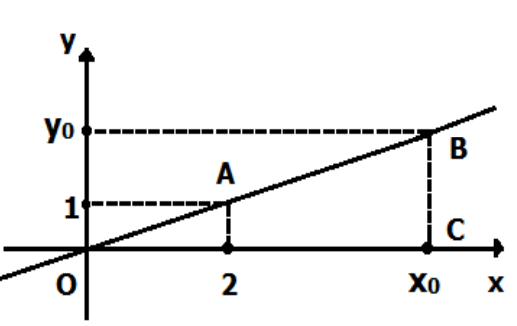
\includegraphics[width=0.35\textwidth]{ds4-b5.png}$$
    Trong hình bên, đường thẳng $\mathrm{OA}$ là đồ thị của hàm số $\mathrm{y}=\mathrm{f}(\mathrm{x})=\mathrm{ax}$.
    \begin{enumerate}[a.]
        \item  Tính tỉ số $\frac{\mathrm{y}_0-2}{\mathrm{x}_0-4}$.
        \item Giả sử $x_0=5$. Tính diện tích tam giác $\mathrm{OBC}$
    \end{enumerate}
    \loigiai{
        \begin{enumerate}
            \item  Điểm $\mathrm{A}$ thuộc đồ thị hàm số $\mathrm{y}=$ ax nên tọa độ $(2 ; 1)$ của A phải thỏa mãn hàm số $\mathrm{y}=\mathrm{ax}$.\\
            Do đó, $1=a .2 \Rightarrow a=\frac{1}{2}$. Vậy hàm số được cho bởi công thức $y=\frac{1}{2} \mathrm{x}$.\\
            Hai điểm $A$ và $B$ thuộc đồ thị hàm số nên hoành độ và tung độ của chúng tỉ lệ thuận với nhau.\\
            Suy ra $\frac{y_0}{x_0}=\frac{1}{2}=\frac{2}{4}=\frac{y_0-2}{x_0-4}$ (theo tính chất của dãy tỉ số bằng nhau)\\
            Vậy $\frac{y_0-2}{x_0-4}=\frac{1}{2}$.
            \item Nếu $x_0=5$ thì $y_0=\frac{1}{2} x_0=\frac{5}{2}=2,5$.\\
            Diện tích tam giác $\mathrm{OBC}$ là:\\
            Áp dụng công thức $S=\frac{1}{2}$ (a.h) ta có:\\
            $\mathrm{SOBC}=\frac{1}{2} \cdot 5 \cdot 2,5=6,25$.
        \end{enumerate}
    }
\end{bt}